\subsection{Architecture}
\begin{figure}[h!]
	\centering
	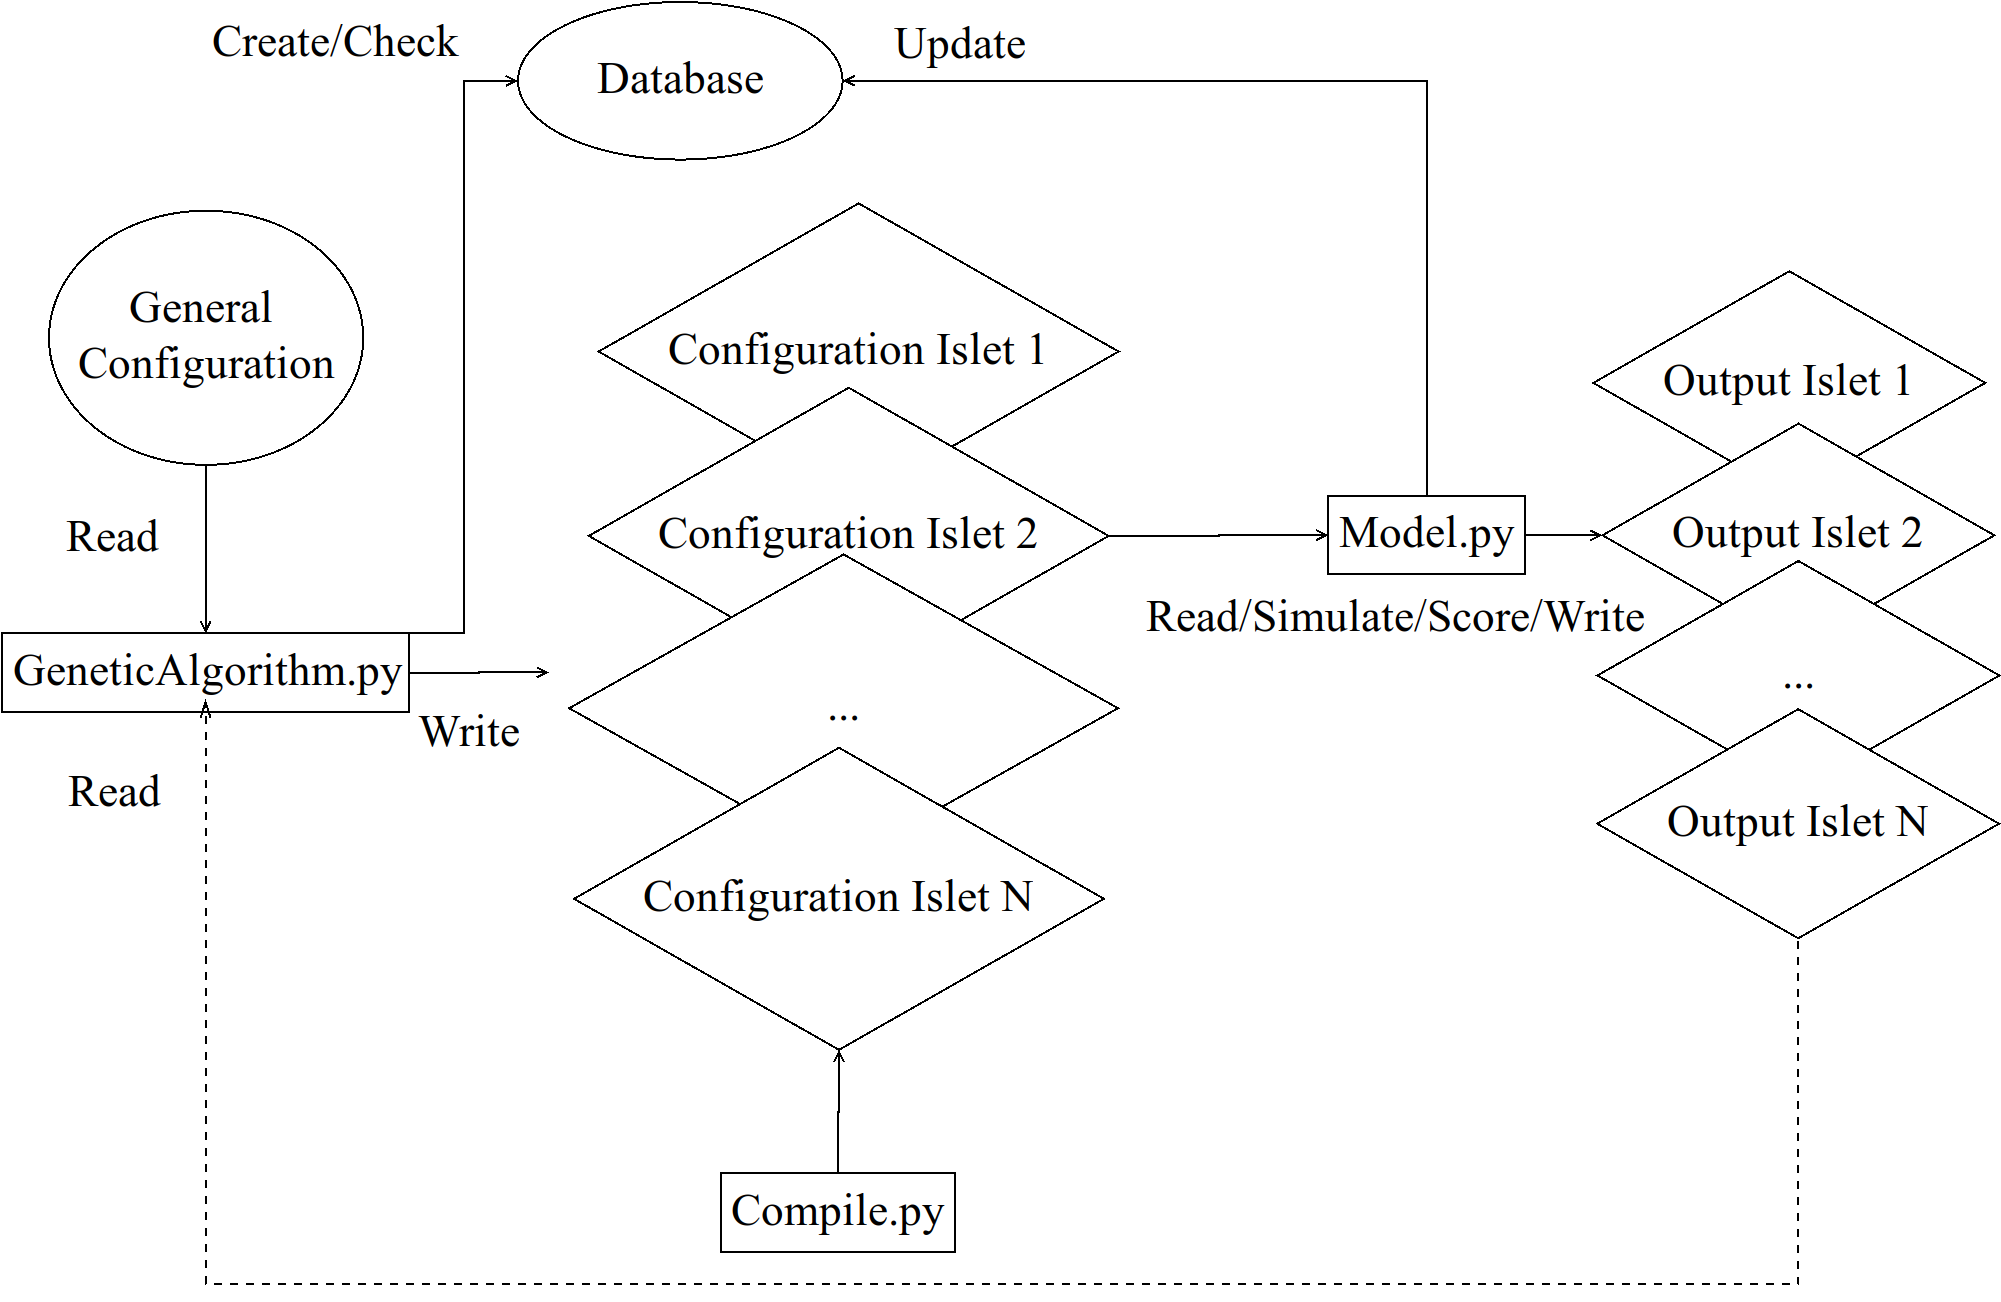
\includegraphics[scale=0.20]{Figures/architecture.png}
	\caption{Architecture of the evolutionary algorithm}
\end{figure}
The evolutionary algorithm is comprised of four recurrent steps: initialization, simulation, selection, and mutation. Initialization consisted of creating configuration files for each cell in an islet according to ranges within which model parameters were allowed to vary and setting up a folder in which appropriate current representations in nmodl would be stored and compiled. Simulation involved reading from the relevant configuration files, transferring control to NEURON to generate data for the given configuration, and scoring the data based on similarity to a reference data set (see the Scoring section). Selection involved passing the highest scoring subset of the current generation's islets to the next generation. The portion of subsequent generations subject to this non-random selection is determined at runtime, and the complementary random subset of the subsequent generation involved creating new configuration files instead of the more commonly used approach of randomly selecting parameters for models from the previous generation. This was done to compensate for the limited scoring metric by increasing randomization. Mutation then changed any parameter that was allowed to vary, randomly within its appropriate range with a probability determined at runtime.
\par Running simulations sequentially, especially with large population sizes and through many generations was significantly slower than running those simulations in parallel. For this reason, a logical structure for the evolutionary algorithm involved the parallelization of computation across simulations. Due to the previously mentioned concerns regarding memory and storage, this parallelization would have to occur with the periodic access to predetermined hardware resources offered by the slurm workload manager in a high performance computing environment. This presented the challenge of unpredictable start times and address spaces for individual simulations. In order for the genetic algorithm to step from one generation to the next, each model instance would have to update some persistent storage to signify its completion and make the relevant details accessible to some independently executed program. A sqlite database was updated to signify simulation completion and store some information regarding model outputs (i.e. score, number of cells, etc.) since the relevant information fit well into the relational model as relational algebra could be used to simplify data processing and organization. Pickle was used to serialize more intricate information regarding model score and comparisons to reference data.

\subsection{Scoring}
\begin{figure}[h!]\label{score}
	\begin{subfigure}{.33\textwidth}
		\centering
		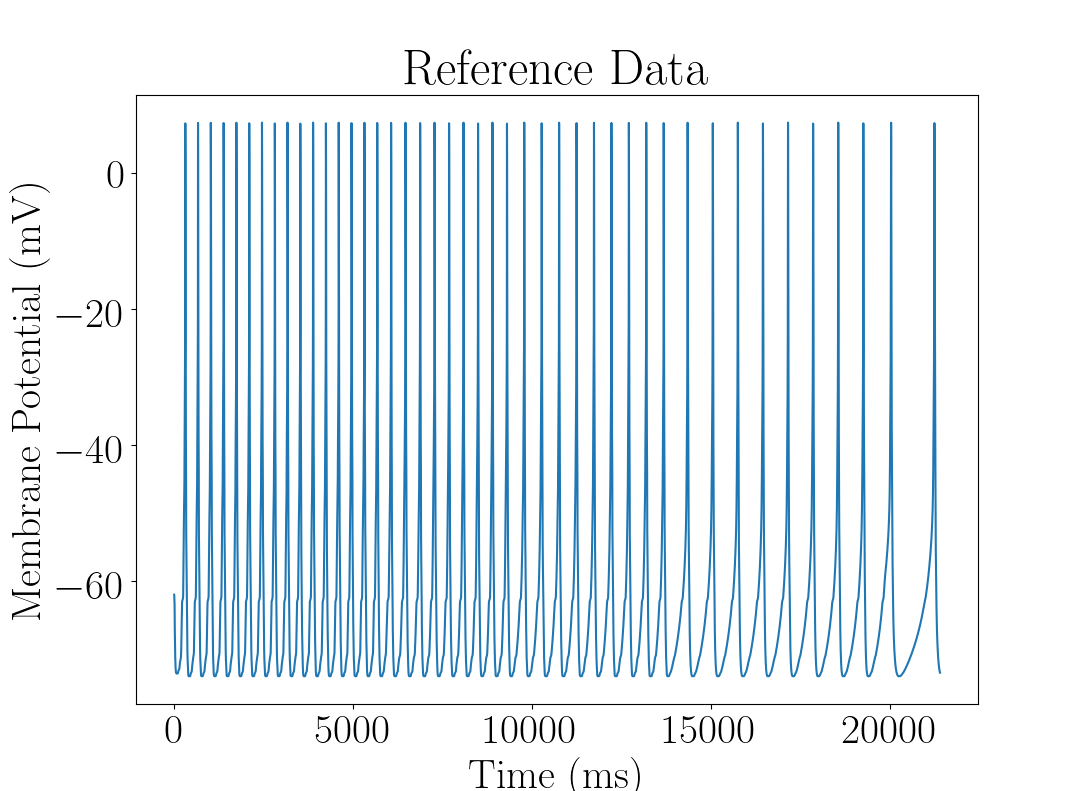
\includegraphics[scale=0.20]{Figures/reference.png}
		\caption{}
		\label{ref}
	\end{subfigure}
	\begin{subfigure}{.33\textwidth}
		\centering
		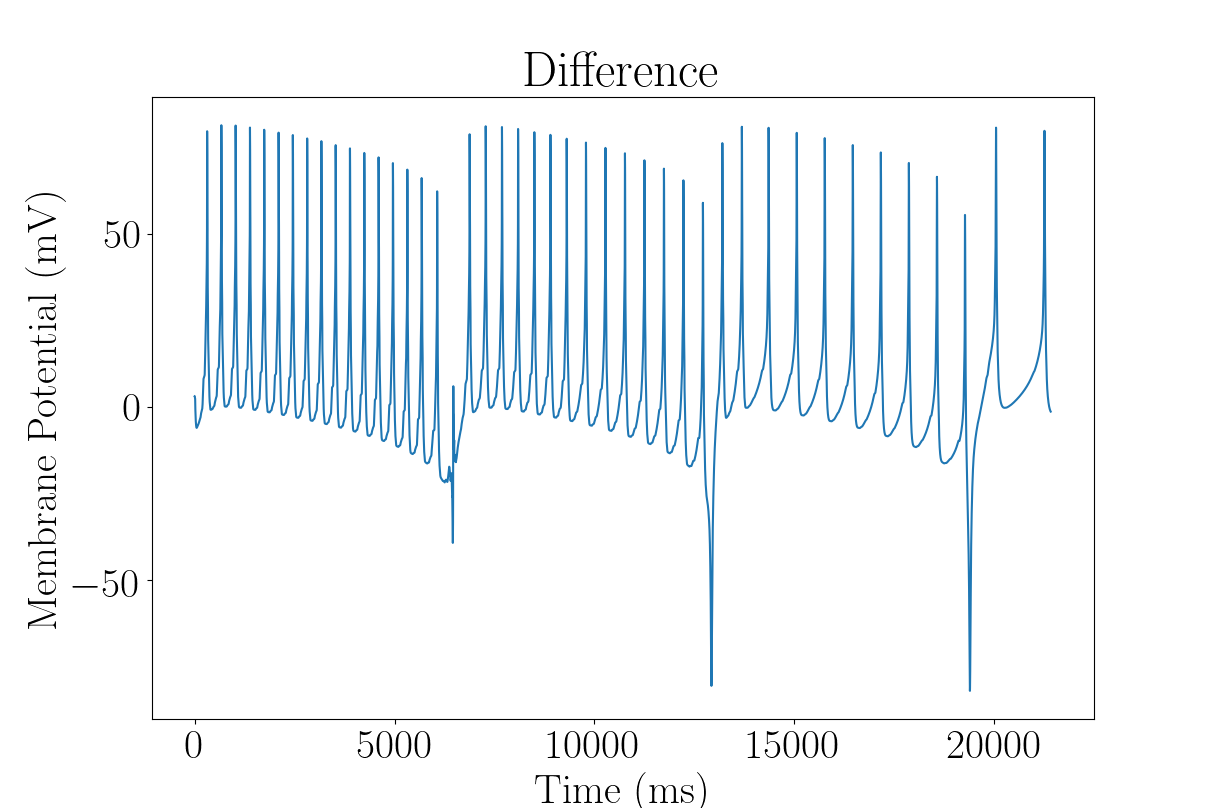
\includegraphics[scale=0.20]{Figures/difference.png}
		\caption{}
		\label{diff}
	\end{subfigure}
	\begin{subfigure}{.33\textwidth}
		\centering
		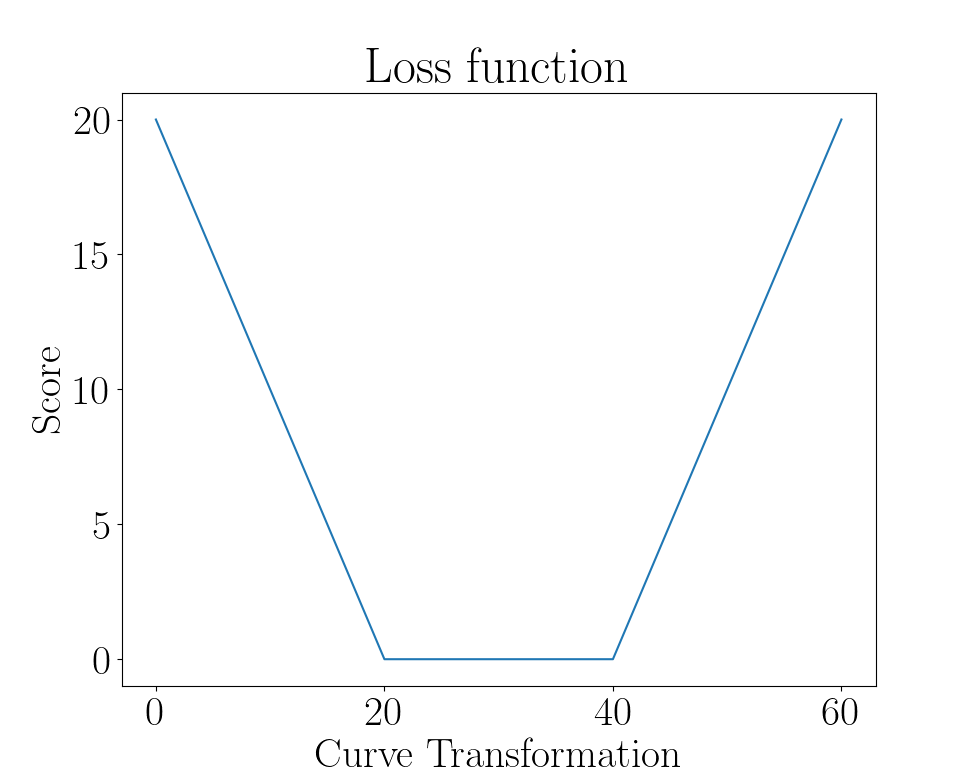
\includegraphics[scale=0.20]{Figures/loss.png}
		\caption{}
		\label{loss}
	\end{subfigure}%
	\caption{Scoring process}
\end{figure}
A strength of this computational model is the flexibility of the data set (i.e. sampling rate, duration, initial conditions) that can be used to parameterize it through the evolutionary algorithm. To best facilitate this flexibility, especially in a future use, the scoring metric and accompanying algorithm were kept simple in this implementation. The sole metric utilized was similarity in the membrane potential time series of simulated $\beta$ cells  to that of a reference data set. Both time series were adjusted such that the sampling rate and duration matched appropriately, and the difference was taken at each point in the simulation. 
\par The scoring process consists of three major steps. The membrane potential of each cell of an islet instance is first normalized to the same time scale that contained the reference data (figure 3a). A difference at each time step is taken between the two data sets and a new time series (figure 3b) is generated. This time series is compressed to a single value by summing all data points and this sum is put through a linear loss function with some threshold (figure 3c). A final sum was completed on the loss output of each compressed time series for each cell of an islet. These scores were compared to each other when instances were evaluated according to how well they reproduced data observed in biological islets. Values that may change the pool of islets selected from a generation (including the median, threshold, and rise of the loss function) were determined at runtime and were the same for all islet instances.